\documentclass{article}
\usepackage[pdftex]{graphicx}
\usepackage{amsmath}

\begin{document}

\section{Levels of Anonymity}
There are three main properties that a anonymization system might want to satisfy.

NOTES: Lets cross-check this against the literature.
\subsection{Requester Anonymity}
The server cannot determine the identity of the client.
\subsection{Provider Anonymity}
Clients cannot determine who is providing they content they download.
\subsection{Sender-Receiver Unlinkability}
An adversary with some level of knowledge of the whole system cannot determine who is communicating with whom.
\subsection{Data Privacy}
Any proxies invovled have no way of figuring out the data.  This will of course require that the client get some sort of public key for the server.
\subsection{Server Unaware}
The server is unaware that it is being commuicated with via a proxy.
\section{Scenarios}
In this section, we present scenarios that would warrant the properties above.
\subsection{End-to-End Connection}
Consider the case where there are two clients within a largely adversarial system that each know the others' address and public key, but who wish to exchange messages without their communication being detected.  That is, they recquire sender-reciever unlinkability.  We will assume that the ADs surrounding each client are definitely untrustworthy.
\subsection{Unsecure Chat Room}
Consider the case of a dissident blogger in a hostile nation wanting to connect to a blogging service.  Obviously, they don't want their password to be visible to the proxy service, nor do they want the proxy service to be able to interfere with the communication.  More importantly, they also want to be anonymous to the service and their communication to be unlinkable to their AD.


\section{General Approaches}
\subsection{Proxy}
The simplest form of requester anonymity is given by a single proxy.  The idea is simple: a trusted third-party will act as a proxy for an entity, forwarding its requests and rerouting the responses, thereby shielding the identity of that entity to the outside, as well as hiding the provider's identity to the requester's AD (assuming it is not also the proxy's AD).  This can be overcome by an adversary with global information by discovering the communications of a proxy and associating that with communications between the proxy and other entities.  This also recquires that the proxy have some sort of incentive to participate.  In the current internet, this incentive is provided sometimes by monetary exchange, and sometimes by the opportunity to intercept the communication and insert advertisements.  If the proxy is compromised, then a single proxy provides no anonymity.
\subsection{Onion Routing and MIXes}
The main idea behind onion routing is to apply the proxy concept several times.  Messages are routed through a series of proxies, thereby making the linking problem much more difficult.  Importantly, even if one or several points in the route are compromised, the total anonymity is not.
\subsection{Broadcast}
Just send your packet to everyone and no one will know who the intended recipient was.  This is in some ways sufficient for reciever anonymity.  


\section{XIA}
\label{sec:xia-overview}
Some features of XIA have implications when it comes to anonymity. We briefly describe the key ideas here and discuss their impact on anonymous communication later.
\subsection{Principal-Based Communication}
In contrast with today's host-based Internet, XIA provides a framework for communication among \emph{principals}. The idea of principal-based communication is that users should be able to address packets directly to their final \emph{intent}. For example, a user searching for books on Amazon wishes to communicate with \texttt{www.amazon.com}; he doesn't care which particular Amazon server responds to his request.

In this example, \texttt{www.amazon.com} can be viewed as a \emph{service} principal. In the case where communication with a particular machine truly is the intent, traditional host-based communication can still be achieved via the \emph{host} principal. Other principals include static \emph{content} (e.g. images) and \emph{autonomous domains} (similar to today's autonomous systems).
\subsection{Intrinsic Security}
All addresses (or, better put, identifiers) in XIA are \emph{intrinsically secure}; exactly what this means varies among principals. For example, a content identifier (CID) is the cryptographic hash of the content itself, enabling anyone receiving the content to verify its integrity. Hosts and services are required to have a public/private key pair; therefore their corresponding identifiers (HIDs and SIDs) are simply the hashes of public keys. A host can sign any communication it generates with its private key and anyone can publicly verify the signature using the host's ID.

The use of identifiers which are cryptographically derived from a user's public key naturally has implications concerning anonymity (or lack thereof) which we discuss further in \S\ref{sec:xia-challenges}.


\section{Adapting Existing Methods for XIA}
In this section we discuss how existing approaches work in XIA.
\subsection{AD-Provided Proxy}
AD routes based on SID, which we trust them not to link to us.
\subsection{Bound-Route Proxy Service}
Your requests all take the same route.
\subsection{Altruistic Onion Routing}
How should Tor work in an XIA setting?


\section{New Approaches Made Possible by XIA}
\subsection{Multi-Route Proxy Service}
In \S\ref{sec:xia-overview} we introduced the service principal. We gave the example of a user communicating with \texttt{www.amazon.com}; in this case, his true intent is to send requests to the Amazon service, not to a particular Amazon server. He addresses his requests to \texttt{www.amazon.com}'s SID and lets the network pick a particular server.

Now consider a similar situation in which a user routes to-be-anonymized packets through a proxy \emph{service} rather than a particular proxy server. Each packet is addressed to SID$_{proxy}$ and is routed by the network to various hosts providing the service (Figure~\ref{fig:proxy-service}). Even if only one proxy server is used per packet, simply by using the the service principle our anonymous user has made it harder for network traffic analysis to discover his use of a proxy.
\begin{figure}
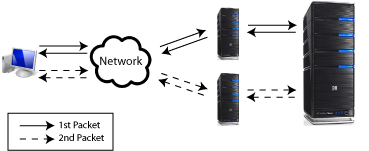
\includegraphics{images/proxy_service_multip_path.png}
\caption{The client routes all requests to SID$_{proxy}$. The network selects a server implementing SID$_{proxy}$ for each packet.}
\label{fig:proxy-service}
\end{figure}

\subsection{The Content Principal}
Something about publishing anonymously?

\subsection{Temporary SIDs from AD}

\subsection{Anonymizing CIDs via a Service}

\section{Challenges Posed by XIA}
\label{sec:xia-challenges}
While XIA provides new mechanisms we can harness for anonymization, some features of the new architecture also introduce challenges to providing anonymity.
\subsection{XIDs are inherently non-anonymous}

\subsection{The trouble with SIDs}
In this section we talk about the "I'll only encrypt with the addressee public key" pitfall.


\section{Accountability?}

\end{document}